%%%%%%%%%%%%%%%%%%%%%%%%%%%%%%%%%%%%%%%%%
% Frequently Asked Questions
% LaTeX Template
% Version 1.0 (22/7/13)
%
% This template has been downloaded from:
% http://www.LaTeXTemplates.com
%
% Original author:
% Adam Glesser (adamglesser@gmail.com)
%
% License:
% CC BY-NC-SA 3.0 (http://creativecommons.org/licenses/by-nc-sa/3.0/)
%
%%%%%%%%%%%%%%%%%%%%%%%%%%%%%%%%%%%%%%%%%

\documentclass[10pt]{article}

\usepackage[margin=0.9in]{geometry} % Required to make the margins smaller to fit more content on each page
\usepackage[linkcolor=blue]{hyperref} % Required to create hyperlinks to questions from elsewhere in the document
\hypersetup{pdfborder={0 0 0}, colorlinks=true, urlcolor=blue} % Specify a color for hyperlinks
\usepackage{todonotes} % Required for the boxes that questions appear in
\usepackage{tocloft} % Required to give customize the table of contents to display questions
\usepackage{microtype} % Slightly tweak font spacing for aesthetics
\usepackage{palatino} % Use the Palatino font
\usepackage{graphicx}
\usepackage{wasysym}
\usepackage{tabularx}
\setlength\parindent{0pt} % Removes all indentation from paragraphs
\setlength\headheight{23pt} 
\usepackage[export]{adjustbox}

% Create and define the list of questions
\newlistof{questions}{faq}{\large List of Frequently Asked Questions} % This creates a new table of contents-like environment that will output a file with extension .faq
\setlength\cftbeforefaqtitleskip{6em} % Adjusts the vertical space between the title and subtitle
\setlength\cftafterfaqtitleskip{1em} % Adjusts the vertical space between the subtitle and the first question
\setlength\cftparskip{.3em} % Adjusts the vertical space between questions in the list of questions
\usepackage{fancyhdr}
\renewcommand{\headrulewidth}{0pt}
\pagestyle{fancy}
\definecolor{314blue}{HTML}{00ADEF}
\definecolor{314orange}{HTML}{F1592A}
\definecolor{lightblue}{HTML}{b2ddd9}
% Create the command used for questions
\newcommand{\question}[1] % This is what you will use to create a new question
{
\refstepcounter{questions} % Increases the questions counter, this can be referenced anywhere with \thequestions
\par\noindent % Creates a new unindented paragraph
\phantomsection % Needed for hyperref compatibility with the \addcontensline command
\addcontentsline{faq}{questions}{#1} % Adds the question to the list of questions
\todo[inline, color=lightblue]{\textbf{#1}} % Uses the todonotes package to create a fancy box to put the question
\vspace{1em} % White space after the question before the start of the answer
}

% Uncomment the line below to get rid of the trailing dots in the table of contents
%\renewcommand{\cftdot}{}

% Uncomment the two lines below to get rid of the numbers in the table of contents
%\let\Contentsline\contentsline
%\renewcommand\contentsline[3]{\Contentsline{#1}{#2}{}}

\begin{document}
\pagenumbering{gobble}
%----------------------------------------------------------------------------------------
%	TITLE AND LIST OF QUESTIONS
%----------------------------------------------------------------------------------------

{\Huge \bf \emph{Individual Donor Analysis: CA-25}} % Main title

{{\it This memo breaks down the individual donors to three campaigns for the CA-25 House seat (Jess Phoenix, Bryan Caforio, and Steve Knight). The data was collected via the FEC database\footnote{\tt{https://www.fec.gov/data/candidate/H8CA25082/}} which releases data every quarter, and covers the final three quarters of 2017. The data was processed to consolidate multiple donations by a single person, except where noted. The identity of many donors is hidden behind a PAC, so I did my best to remove PAC contributions, aside from those from ActBlue. Any contribution of more than \$2,700 was also assumed not to come from an individual and was ignored.}}

%\newpage % Comment this if you would like your questions and answers to start immediately after table of questions

%----------------------------------------------------------------------------------------
%	QUESTIONS AND ANSWERS
%----------------------------------------------------------------------------------------

\question{Donor Distribution: Overall}\label{new-question}

{\Large \bf{Phoenix}}

Jess Phoenix had 313 unique donors (including herself) and raised a total of \$168,296.02 for a mean donation of \$537.69 per donor, with a median donation of \$250.00. 
The table below displays the number of donors in each of 5 monetary bins and the total amount raised in those bins, and the same data in two pie charts is shown below the table for a visual comparison.

\begin{table}[ht]
\begin{tabularx}{\textwidth}{c | c c | c c}
 \bf{Donation Amount} & \bf{Number of Donors} & \bf{Percentage of Total} & \bf{Amount Donated} & \bf{Percentage of Total} \\ \hline
\enspace \enspace \enspace \$0-\$100 &\quad \quad \quad 66 & 21.1\% &\quad \quad  \$3,522.00 & 2.1\%\\ \hline
\enspace \enspace \enspace \$100-\$250 &\quad \quad \quad \ 100 & 31.9\% &\quad \quad \$23,992.00 & 14.5\% \\ \hline
\enspace \enspace \enspace \$250-\$500 &\quad \quad \quad \ 81 & 25.9\% &\quad \quad\$34,758.30 & 21.1\%\\ \hline
\enspace \enspace \enspace \$500-\$2,000 &\quad \quad \quad \ 44 & 14.1\% &\quad \quad \$46247.77 & 28.0\%\\ \hline
\enspace \enspace \enspace \$2,000-\$2,700 &\quad \quad \quad \ 22 & 7.0\% &\quad \quad \$56,500.00 & 34.2\% \\ \hline
\bf{Totals} & \quad \quad \quad 317 & & \quad \quad \$172078.74 &\\  
\end{tabularx}
\end{table}
\begin{figure}[ht]
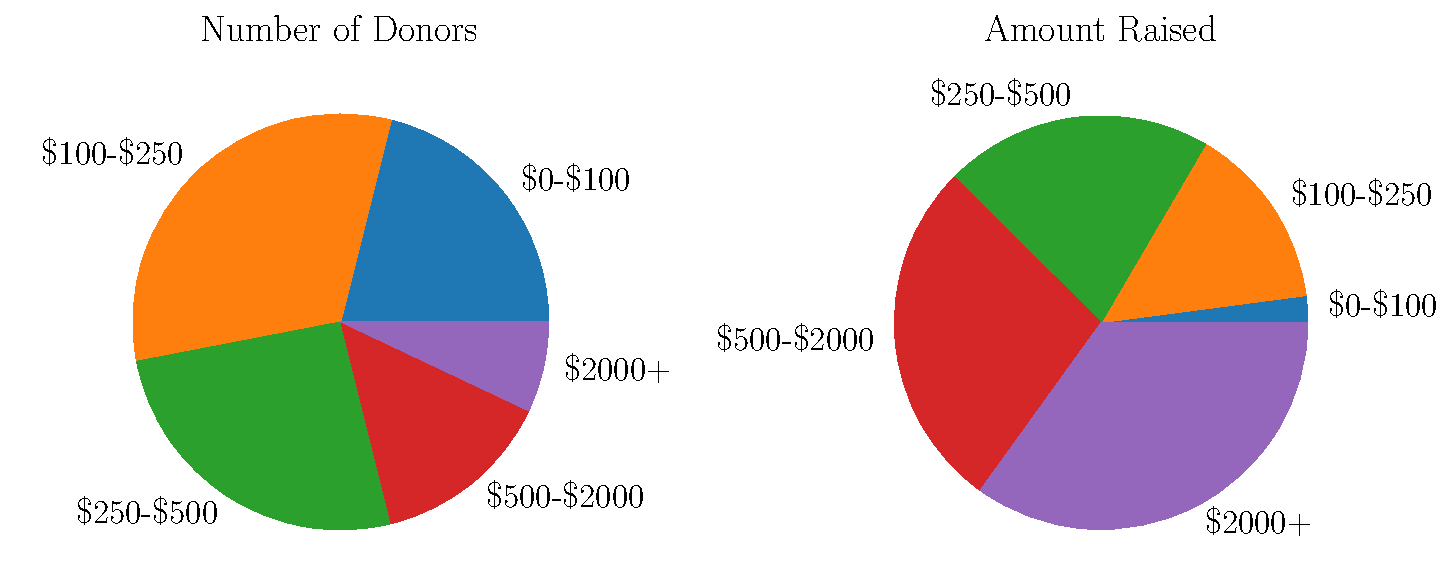
\includegraphics[width=0.8\linewidth, center]{Phoenix_Totals.pdf}
\caption{Jess Phoenix overall donation distribution from individuals}
\end{figure}

{\Large \bf{Caforio}}

Bryan Caforio had 1275 unique donors (including himself) and raised a total of \$562,725.41 for a mean donation of \$441.35 per donor. The median donation was \$250.00. 

\begin{table}[ht]
\begin{tabularx}{\textwidth}{c | c c | c c}
 \bf{Donation Amount} & \bf{Number of Donors} & \bf{Percentage of Total} & \bf{Amount Donated} & \bf{Percentage of Total} \\ \hline
\enspace \enspace \enspace \$0-\$100 &\quad \quad \quad 392 & 30.7\% &\quad \quad  \$18,738.04 & 3.3\%\\ \hline
\enspace \enspace \enspace \$100-\$250 &\quad \quad \quad \ 353 & 27.7\% &\quad \quad \$84,091.00 & 14.9\% \\ \hline
\enspace \enspace \enspace \$250-\$500 &\quad \quad \quad \ 294 & 23.1\% &\quad \quad\$139,210.41 & 24.7\%\\ \hline
\enspace \enspace \enspace \$500-\$2,000 &\quad \quad \quad \ 192 & 15.1\% &\quad \quad \$204,944.0016 & 36.4\%\\ \hline
\enspace \enspace \enspace \$2,000-\$2,700 &\quad \quad \quad \ 44 & 3.5\% &\quad \quad \$115,741.80 & 20.6\% \\ \hline
\bf{Totals} & \quad \quad \quad 1275 & & \quad \quad \$562,725.41 &\\  
\end{tabularx}
\end{table}
\begin{figure}[h]
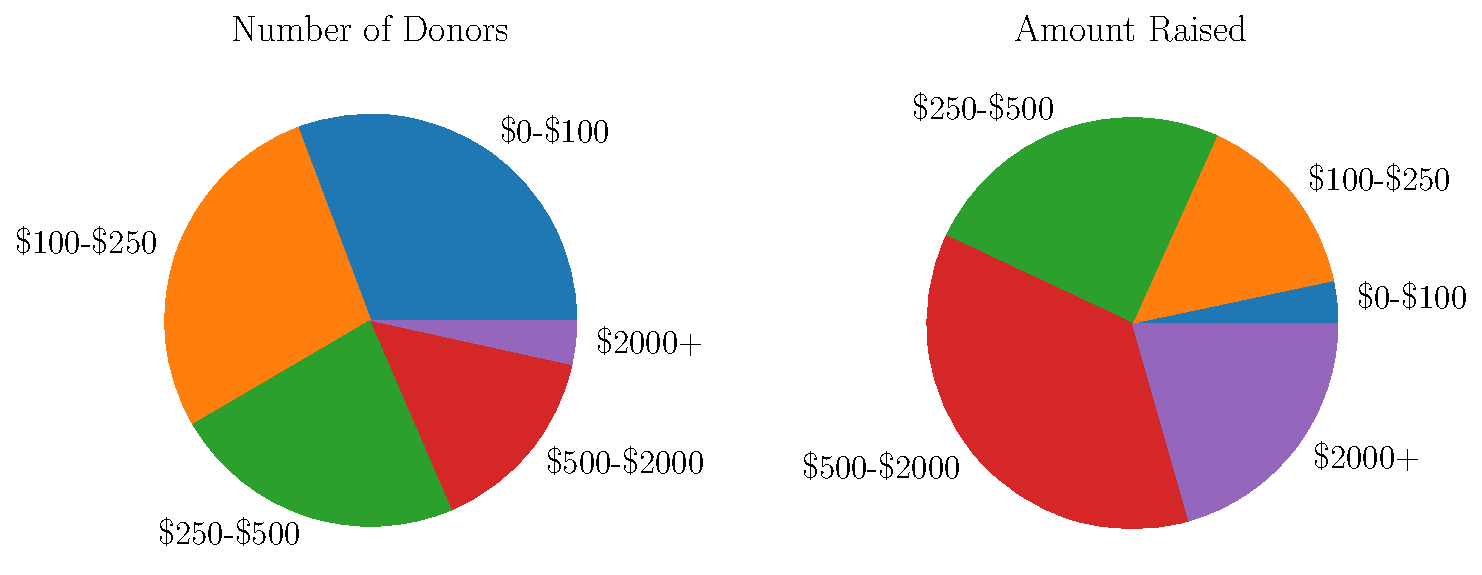
\includegraphics[width=0.8\linewidth, center]{Caforio_Totals.pdf}
\caption{Bryan Caforio overall donation distribution from individuals}
\end{figure}

{\Large \bf{Knight}}

Steve Knight had 180 unique donors and raised a total of \$190,898.28 for a mean donation of \$1,060.55 per donor. The median donation was \$782.14. A large portion of Steve Knight's donations come from PACs instead of from individuals, which is why the amounts shown below are significantly below those seen in the time-series data below. 

\begin{table}[ht]
\begin{tabularx}{\textwidth}{c | c c | c c}
 \bf{Donation Amount} & \bf{Number of Donors} & \bf{Percentage of Total} & \bf{Amount Donated} & \bf{Percentage of Total} \\ \hline
\enspace \enspace \enspace \$0-\$100 &\quad \quad \quad 2 & 1.1\% &\quad \quad  \$150.00 & 0.07\%\\ \hline
\enspace \enspace \enspace \$100-\$250 &\quad \quad \quad \ 23 & 12.8\% &\quad \quad \$5,575.00 & 2.9\% \\ \hline
\enspace \enspace \enspace \$250-\$500 &\quad \quad \quad \ 61 & 33.9\% &\quad \quad\$30,150.00 & 15.8\%\\ \hline
\enspace \enspace \enspace \$500-\$2,000 &\quad \quad \quad \ 65 & 36.1\% &\quad \quad \$80,314.28 & 42.1\%\\ \hline
\enspace \enspace \enspace \$2,000-\$2,700 &\quad \quad \quad \ 29 & 16.1\% &\quad \quad \$74,709.00 & 39.1\% \\ \hline
\bf{Totals} & \quad \quad \quad 180 & & \quad \quad \$190,898.28 &\\  
\end{tabularx}
\end{table}
\begin{figure}[ht]
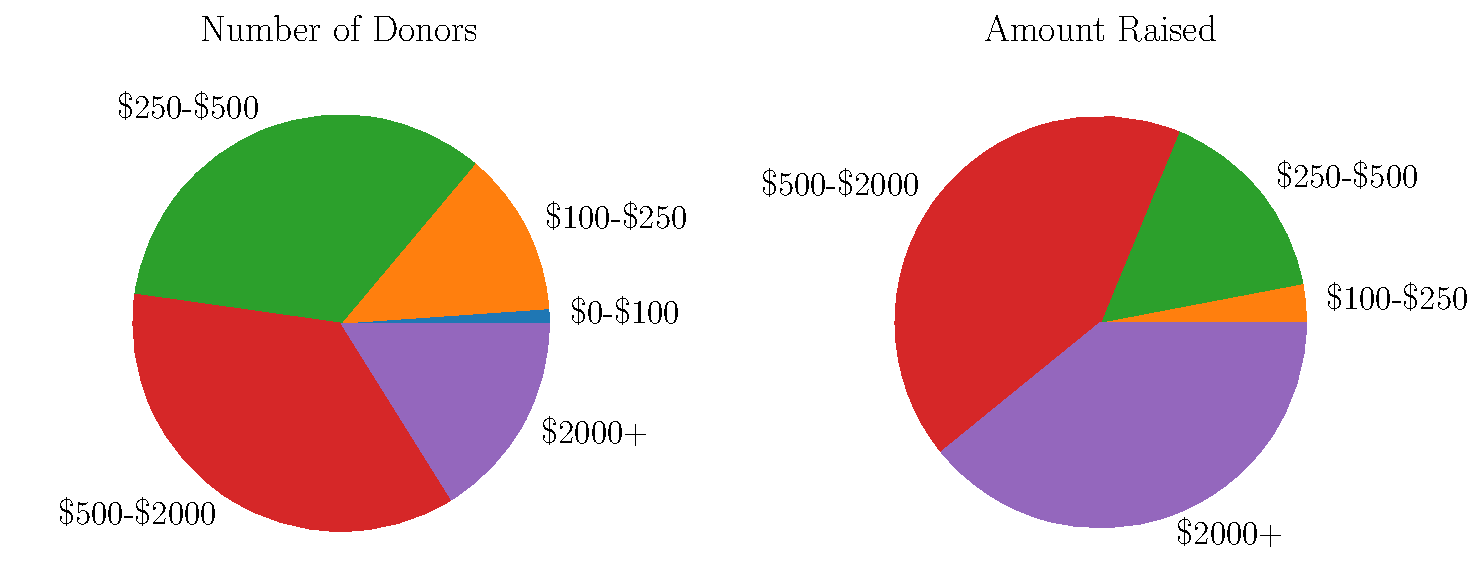
\includegraphics[width=0.8\linewidth, center]{Knight_Totals.pdf}
\caption{Steve Knight overall donation distribution from individuals}

\end{figure}


\question{In-District vs. Out-of-District}\label{district}

{\Large \bf{Phoenix}}

Jess Phoenix had 5 in-district donors (1.6\% of all donors) who combined for a total of \$3,275.95 (1.9\% of her total). Her out-of-district donors combined for a large majority of her donations- 308 (98.4\%) donors combined for \$165,020.07 (98.1\% of her total). I won't break down the data further here, since it is so similar to her overall donor distribution above.


{\Large \bf{Caforio}}

Bryan Caforio had 153 in-district donors (12\% of all donors) who combined for a total of \$35,201.48 (6.3\% of his total). He had 1,122 (88\%) donors from outside his district, who combined for \$527,523.93 (93.7\% of his total). The breakdown is presented below:

\begin{table}[ht]
\begin{tabularx}{\textwidth}{c | c c | c c}
\multicolumn{5}{l}{\bf{In-district}} \\ \hline
 \bf{Donation Amount} & \bf{Number of Donors} & \bf{Percentage of Total} & \bf{Amount Donated} & \bf{Percentage of Total} \\ \hline
\enspace \enspace \enspace \$0-\$100 &\quad \quad \quad 95 & 7.5\% &\quad \quad  \$5787.68 & 1.0\%\\ \hline
\enspace \enspace \enspace \$100-\$250 &\quad \quad \quad \ 23 & 1.8\% &\quad \quad \$4166.00 & 0.7\% \\ \hline
\enspace \enspace \enspace \$250-\$500 &\quad \quad \quad \ 22 & 1.7\% &\quad \quad\$9,181.77 & 1.6\%\\ \hline
\enspace \enspace \enspace \$500-\$2,000 &\quad \quad \quad \ 12 & 0.9\% &\quad \quad \$13366.03 & 2.4\%\\ \hline
\enspace \enspace \enspace \$2,000-\$2,700 &\quad \quad \quad \ 1 & 0.07\% &\quad \quad \$2,700.00 & 0.5\% \\ \hline
\bf{Totals} & \quad \quad \quad \bf{153} & \bf{12.0\%} & \quad \quad \bf{\$35,201.48} & \bf{6.3\%} \\  
\hline \hline
\multicolumn{5}{l}{\bf{Out-of-district}} \\ \hline
\enspace \enspace \enspace \$0-\$100 &\quad \quad \quad 297 & 23.3\% &\quad \quad  \$12,950.36 & 2.3\%\\ \hline
\enspace \enspace \enspace \$100-\$250 &\quad \quad \quad \ 330 & 25.9\% &\quad \quad \$79,925.00 & 14.2\% \\ \hline
\enspace \enspace \enspace \$250-\$500 &\quad \quad \quad \ 272 & 21.3\% &\quad \quad\$130,028.64 & 23.1\%\\ \hline
\enspace \enspace \enspace \$500-\$2,000 &\quad \quad \quad \ 180 & 14.1\% &\quad \quad \$191,578.13 & 34.0\%\\ \hline
\enspace \enspace \enspace \$2,000-\$2,700 &\quad \quad \quad \ 43 & 3.4\% &\quad \quad \$113,041.80 & 20.1\% \\ \hline
\bf{Totals} & \quad \quad \quad \bf{1122} & \bf{88\%} & \quad \quad \bf{\$527,523.93} & \bf{93.7\%}\\  

\end{tabularx}
\end{table}

{\Large \bf{Knight}}

Steve Knight had 32 in-district donors (17.8\% of all donors) who combined for a total of \$33,550.00 (17.6\% of his total). He had 148 (82.2\%) donors from outside his district, who combined for \$157,348.28 (82.4\% of his total). The breakdown is presented below:

\begin{table}[ht]
\begin{tabularx}{\textwidth}{c | c c | c c}
\multicolumn{5}{l}{\bf{In-district}} \\ \hline
 \bf{Donation Amount} & \bf{Number of Donors} & \bf{Percentage of Total} & \bf{Amount Donated} & \bf{Percentage of Total} \\ \hline
\enspace \enspace \enspace \$0-\$100 &\quad \quad \quad 2 & 1.1\% &\quad \quad  \$150.00 & 0.08\%\\ \hline
\enspace \enspace \enspace \$100-\$250 &\quad \quad \quad \ 3 & 1.7\% &\quad \quad \$700.00 & 0.4\% \\ \hline
\enspace \enspace \enspace \$250-\$500 &\quad \quad \quad \ 11 & 6.1\% &\quad \quad\$5,500.00 & 2.9\%\\ \hline
\enspace \enspace \enspace \$500-\$2,000 &\quad \quad \quad \ 10 & 5.6\% &\quad \quad \$12,200.00 & 6.4\%\\ \hline
\enspace \enspace \enspace \$2,000-\$2,700 &\quad \quad \quad \ 6 & 3.3\% &\quad \quad \$15,000.00 & 7.9\% \\ \hline
\bf{Totals} & \quad \quad \quad \bf{32} & \bf{17.8\%} & \quad \quad \bf{\$33,550.00} & \bf{17.6\%} \\  
\hline \hline
\multicolumn{5}{l}{\bf{Out-of-district}} \\ \hline
\enspace \enspace \enspace \$0-\$100 &\quad \quad \quad 0 & 0.0\% &\quad \quad  \$0.00 & 0.0\%\\ \hline
\enspace \enspace \enspace \$100-\$250 &\quad \quad \quad \ 20 & 11.1\% &\quad \quad \$4,875.00 & 2.6\% \\ \hline
\enspace \enspace \enspace \$250-\$500 &\quad \quad \quad \ 50 & 27.8\% &\quad \quad\$24,650.00 & 12.9\%\\ \hline
\enspace \enspace \enspace \$500-\$2,000 &\quad \quad \quad \ 55 & 30.6\% &\quad \quad \$68,114.28 & 35.7\%\\ \hline
\enspace \enspace \enspace \$2,000-\$2,700 &\quad \quad \quad \ 23 & 12.8\% &\quad \quad \$59,709.00 & 31.3\% \\ \hline
\bf{Totals} & \quad \quad \quad \bf{148} & \bf{82.2\%} & \quad \quad \bf{\$157,348.28} & \bf{82.4\%}\\  

\end{tabularx}
\end{table}


\question{Temporal distribution of donations}

The number of donations to all three candidates as a function of time shows spikes every three months at the end of the quarter (June 30, September 30, and December 31), as can be seen in the plots below. This may just be a quirk of the fact that those dates are the filing deadlines for FEC data, but there does seem to be an increase in the number of donations for at least a few weeks ahead of each deadline as well. The effect is most pronounced among the biggest donors.

\it{Note: this data has not been processed to consolidate multiple donations made by the same person}

\begin{figure}
  \begin{minipage}[b]{0.45\linewidth}
  \raggedright
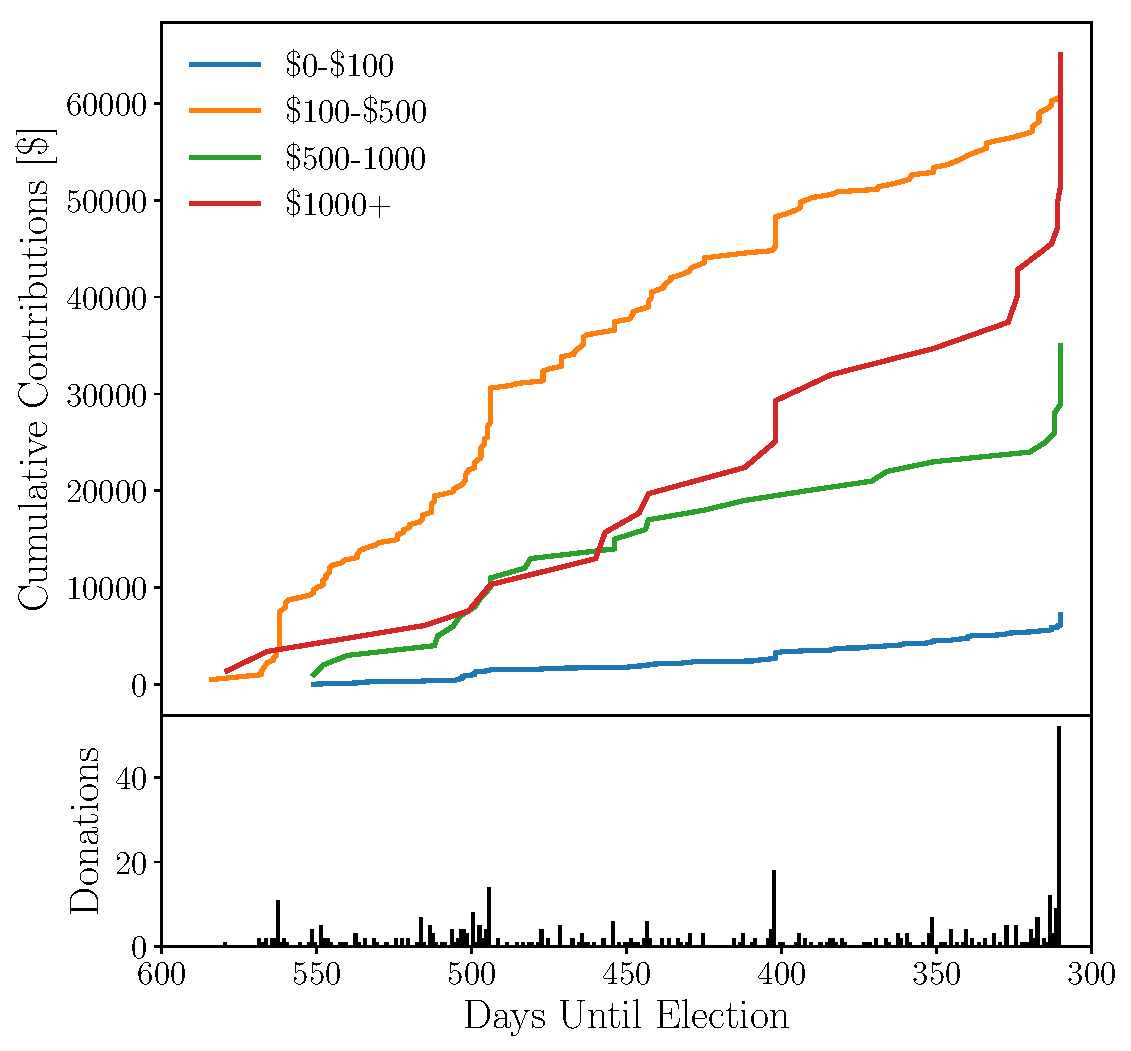
\includegraphics[width=\textwidth, center]{Phoenix_Totals_overTime.pdf}
\caption{Jess Phoenix contributions over time.}
\end{minipage}
  \begin{minipage}[b]{0.45\linewidth}
  \raggedleft
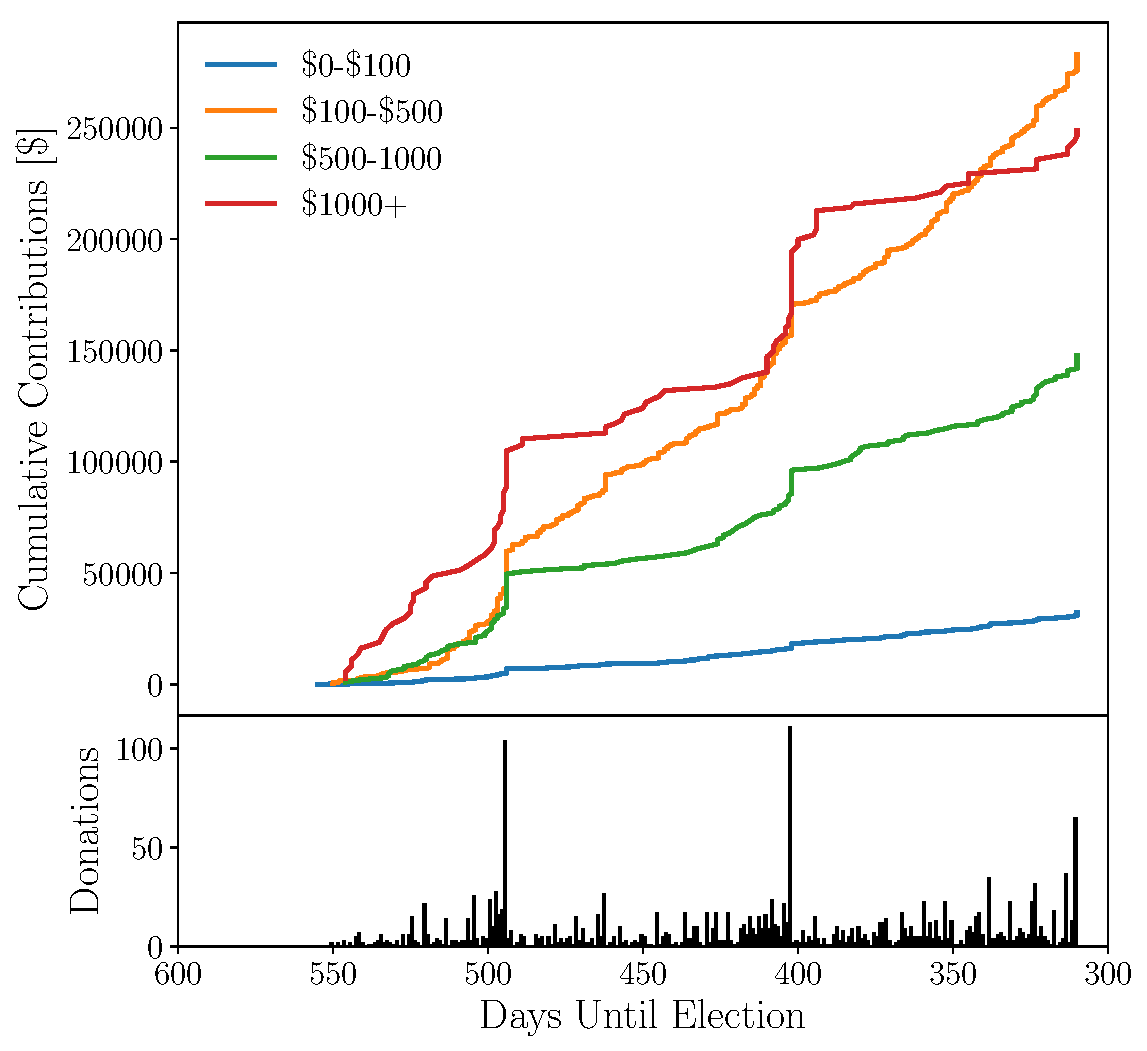
\includegraphics[width=\textwidth, center]{Caforio_Totals_overTime.pdf}
\caption{Bryan Caforio contributions over time.}
\end{minipage}
\end{figure}

\begin{figure}[ht]
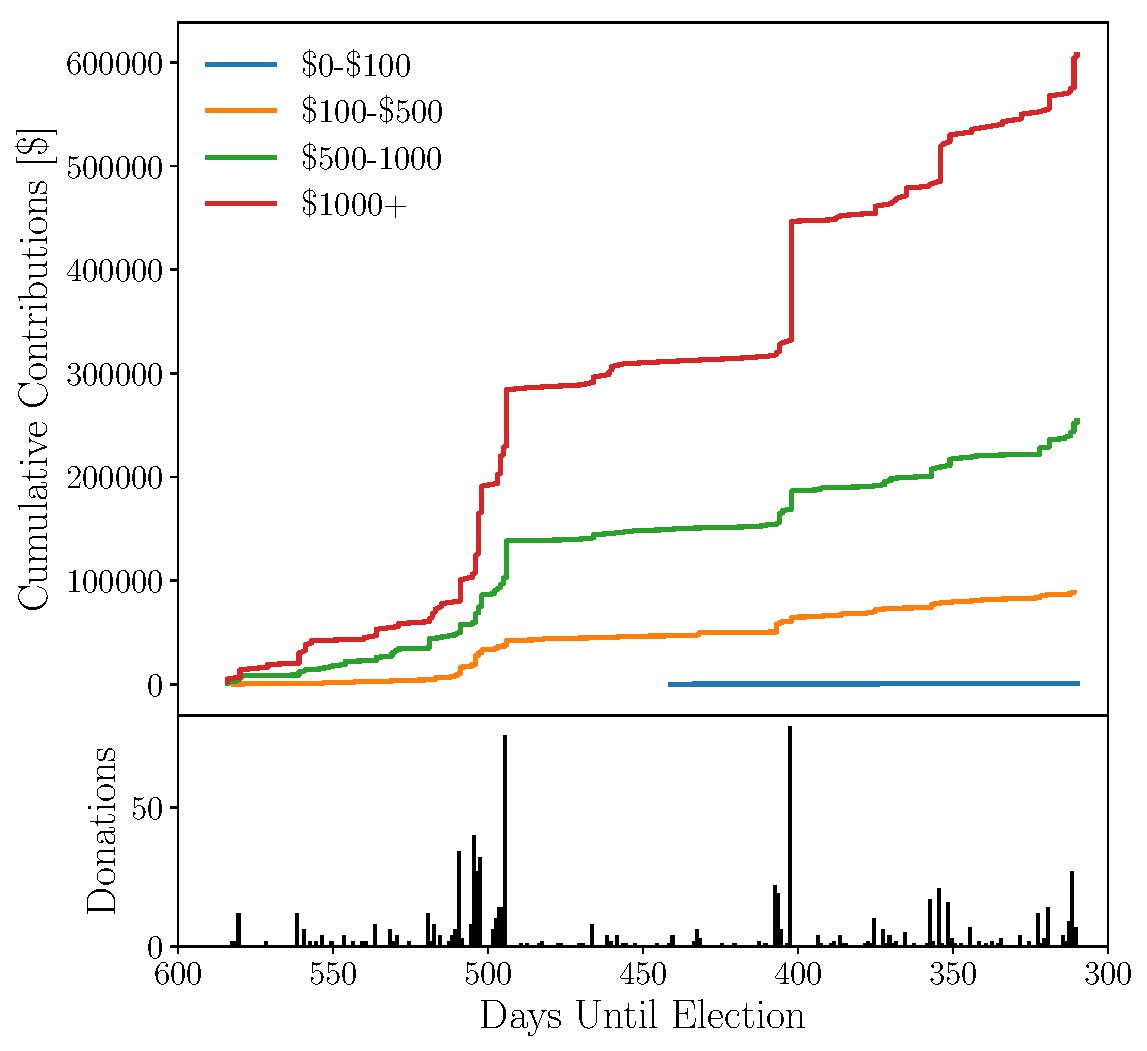
\includegraphics[width=0.5\linewidth, center]{Knight_Totals_overTime.pdf}
\caption{Steve Knight contributions over time.}

\end{figure}



%------------------------------------------------
\end{document}